%=========================================================================
% (c) 2011, 2012 Josef Lusticky

\section{Network communication}
% 1 - see design/network.tex
Communication over IEEE~802.15.4 link layer uses a 6LoWPAN adaptation layer.
Thanks to this layer, AVR Raven running Contiki OS is connected to the IPv6 Internet.
The client and the developed interface uses no IP version specific code,
therefore a communication over IPv4 should be also possible, though not tested.

The packet loss problem was described in section~\ref{sec:design-network}.
However, packet loss is not a matter for NTP if using either broadcast or unicast mode.
In broadcast mode, lost server packet causes no setting or adjusting time of client's
local clock.
The client simply waits without disruption for next NTP broadcast message.
If client needs to figure out it's local clock offset at the moment,
it can simply query a server using NTP unicast mode.
% 2
Upon sending the packet, the NTP client process yields
using the {\it{PROCESS\_YIELD}} statement, so no active waiting
causes blocking the whole system.

The remote NTP server can be specified in Makefile or
using the {\it{REMOTE\_HOST}} define macro.
If no remote host is specified,
NTP client assumes only NTP broadcast communication mode will be used.
The broadcast mode is intended particularly for energy or memory constrained clients
or for a huge number of NTP clients and a single NTP server
in a network with small propagation delay.
Should there be more devices running Contiki present in one network,
each of them needs a different link layer address.
This address can be configured in Makefile as well.
Beware that although the firmware for RZ~USB Stick automatically translates
between Ethernet link layer addresses (MAC addresses) and IEEE~802.15.4 link layer
addresses, both are are still different links and can not be mixed in one
layer~2 network (e.g. bridging will not work).

Dynamic increasing or decreasing the client's poll interval in response to
Kiss-o'-Death packets, described in section~\ref{sec:ntp-network}, is not implemented.
The configuration instead assumes, that an exhausted NTP server rather drops the incoming
client's packet than sending the response with KoD code.

Contiki NTP Client is primarily intended for use in local networks with a single master NTP server,
although using any NTP server found in the Internet would work.
Figure~\ref{fig:implementation-routing} shows the network topology used
for tests and measurements of Contiki NTP Client.
% How to set up the illustrated network is described in tutorial on CD.
The Meinberg primary NTP server was synchronised with PPS %todo.
Measurements made using this setup are discussed in chapter~\ref{chap:measurements}.

\begin{figure}
	\centering
	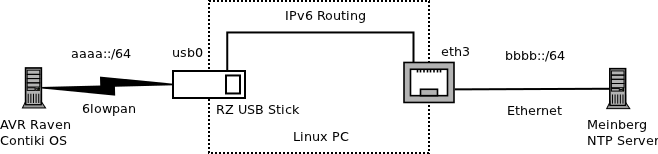
\includegraphics[width=10cm,keepaspectratio]{fig/radvd-routing.png}
	\caption{Contiki NTP Client communicating with remote NTP server}
	\label{fig:implementation-routing}
	%\bigskip
\end{figure}
